\pdfminorversion=7
\documentclass[letterpaper]{article}
\def\name{Daniel Bee}

\title{Social Dynamics in Code Review}
\author{\name}
\date{}

\usepackage{fancyhdr}
\usepackage{geometry}
\usepackage{lastpage}
\usepackage{hyperref}
\usepackage[UKenglish]{isodate}
\usepackage{indentfirst}
\usepackage{graphicx}
\usepackage{cleveref}

% Remove ordinal day reference
\cleanlookdateon

\geometry{
	body={6.0in, 8.5in},
	left=1.1in,
	right=1.1in,
}

\pagestyle{fancy}
\lhead{Research Project Proposal - \name}
\rhead{}
\cfoot{Page \thepage\ of \pageref*{LastPage} - Last updated: \today}

\begin{document}

\begingroup
\noindent
{\bf I am applying for a RHUL PhD Student Purpose Studentship}
\let\newpage\relax%
\maketitle
\endgroup

\thispagestyle{fancy}


\section{How The Project Addresses Social Purpose}
A tremendous number of industries move their operations from the physical world to the digital world.
We are living in the era where the role of software is getting more significant.
As the importance of software grows, the social demands on good quality software also grow.
However, it is still a challenge to develop and maintain good quality software.

The main goal of my research project is to understand and improve the current software engineering practices for social purpose.
Among diverse software engineering practices, I will specifically focus on code review---an auditing process for code changes.
Code review is one of the most outstanding quality assurance practices and heavily rely on social interactions between developers~\cite{Bosu17,Toufique17}.
Unfortunately, existing studies on code review often overlook the social interactions involved in code review.
By conducting empirical studies on social interactions during code review, I believe my research can make a meaningful contribution to the software engineering research community.
For example, these studies can provide deeper insights into Equality, Diversity, and Inclusion (EDI) among participants involved in code review.
Additionally, I expect my research will identify several challenges in code review.
I plan to address these challenges by proposing automated techniques based on my software engineering background.

%Additionally, my research on code review also can help people without expert knowledge in computer science to develop and maintain their own software.
%Recent advancements of Large Language Models (LLMs) have lower the entry barrier to software development for the general public~\cite{Zhou23icpc}.
%Based on my empirical studies, I believe we can gain a deeper understanding of current code review practices across different levels of developers---including the general public---and identify several challenges.
%Finally, I can come up with several automated techniques based on my software engineering background that can mitigate the challenges. 


\section{Project Background}
Code review is an auditing process in which any code changes are reviewed by colleagues rather than the author of the changes.
Recent empirical studies~\cite{Bacchelli13,Mcintosh16} have demonstrated that code review is beneficial in diverse aspects (e.g., finding defects, alternative solutions, and knowledge sharing).
Due to its diverse benefits, despite the additional cost of running the process, it has been widely adopted in both proprietary software development industry and open source projects~\cite{Sadowski18, Mukadam13}.

Although code review inherently involves social interactions between colleagues in a team~\cite{Bosu17,Toufique17}, it is true that not many software engineering studies focus on the importance of these interactions. 
Additionally, recent advancements in Large Language Models (LLMs) have significantly changed code review practices~\cite{Zhou23icpc}.
LLMs support code reviewers to write code review comments and change authors to revise their changes based on review comments. 
Since these supports can significantly reduce manual efforts, many practitioners adopt it in their code review processes.
However, it can reduce the frequency of social interactions between team members, and the impact has not been properly investigated.

As a first step, I have worked with my supervisor, Dr. DongGyun Han, to visualise the social interactions among actors involved in code review.
The project was initially supported by the Department of Computer Science as part of the Undergraduate Research Opportunities programme in 2024.
We submitted this work to the ACM International Conference on the Foundation of Software Engineering (FSE), one of the most prestigious conferences in software engineering (Core A*), and it was accepted in 2025~\cite{Bee25}.
With the generous support of the Department of Computer Science, I was able to present my work at the conference and discuss potential extensions with other participants.
Specifically, I implemented Code Review Visualisation (CRV) framework that 1) collects code review data from a collaborative workspace, 2) migrates the data into an optimised database, and 3) visualises social interactions using a graph-based view.
\Cref{fig:snapshot} shows an example of the visualisation.
In the visualisation, each node represents individual participant.
Its size shows the frequency of their code review comments for the software project.
If two participants left comment within the same code review request, an edge connects them.
The thickness of edge dedicates the normalised frequency how often the two developers discuss within the same code review request.


\begin{figure}[t]
  \centering
  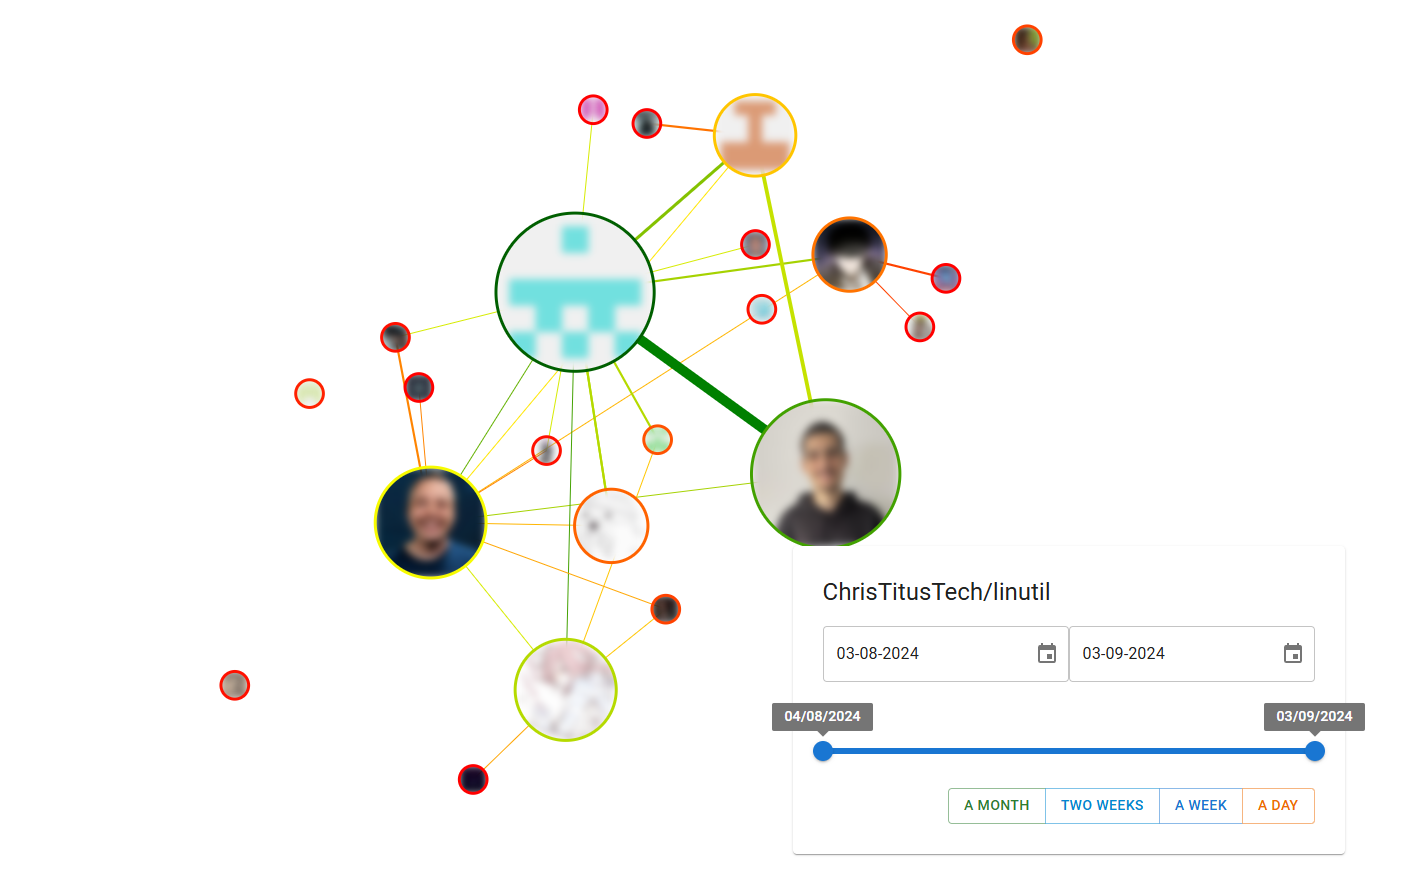
\includegraphics[width=0.8\textwidth]{figures/image.png}
  \caption{An example of visualisation. The profile photos are blurred to protect the participants' privacy~\cite{Bee25}}
  \label{fig:snapshot}
\end{figure}

\section{Aim \& Objective of the Project}

\begin{itemize}
  \item {\bf Understand current practices.} By conducting diverse empirical studies, I expect we will get a better understanding of current practices.
  \item {\bf Identify challenges and potential improvement.} Among the empirical findings, I believe some have the potential to highlight current challenges and improve existing practices.
  \item {\bf Modelling the findings.} By modelling code review practices, I plan to develop automated techniques that can correctly predict potential outcomes of the social interactions between participants.
\end{itemize}


\section{Design of the Research Project}

\noindent
{\bf Systematic Literature Review} (SLR)~\cite{Kitchenham10} will help me to get a thorough and comprehensive understanding on existing studies. 
I will focus on investigating code review studies.
Specifically, the studies about social interactions in code review.
Based on the understanding, I can identify the topics are well-studied and which are under-studied.


\noindent
{\bf Empirical Studies} By using both quantitative and qualitative analyses, I can gain a deeper understanding of existing practices.
I believe the SLR process will reveal several potential topics for empirical studies. 
My first empirical study will be about the usability of CRV.
Although we demonstrated CRV by using several open source projects, its actual usability and contribution to real practice have not yet been investigated.
The objective data from the empirical study will encourage practitioners to adopt CRV more widely.
I believe this, in turn, will lead to increased opportunities for collaboration. 

\noindent
{\bf Modelling}

\section{Planned Timeline}
%Planned timeline for work to be completed; this does not need to be very detailed but should show progression of the work to be completed, including placement, across the 3.5 years

{\bf Year 1.} I will focus on conducting an SLR~\cite{Kitchenham10} to gain a thorough and comprehensive understanding of existing studies in the domain and refine my research plan.
Simultaneously, I will conduct an empirical study on CRV as I am already working on it.
This will bring me a good experience to exercise academic writing.

{\bf Year 2--3.} I expect to identify potential research topics via SLR in Year 1.
As mentioned above, I will conduct two lines of research: empirical studies and developing automated techniques to enhance code review practices.

{\bf Year 3--3.5.} I believe my research outputs have now become clear and are ready to be shared with practitioners.
I will contact potential industry partners or open source projects to replicate my empirical studies.
Additionally, if I can successfully manage to develop automated techniques, I will conduct an empirical study on their usability in real practice.


\section{Supervision Team}
%Outline supervision team and what each will bring to the project

\noindent
{\bf Dr. DongGyun Han}

Dr. Han will be the primary supervisor of my PhD project.
He has a strong background in both academia and industry.
Specifically, his experience in empirical software engineering and code review research will support me in carrying out the project.


\noindent
{\bf Dr. Francisco Ferreira}

Dr. Ferreira will be the secondary supervisor.
He is an expert in type systems and formal logic.
I expect his expertise in these areas will help me model social interactions between participants in code review.
Based on this model, I believe I can develop automated techniques to improve the current code review practices.



\section{Additional Research Support}
%Details on any research funding support that will be required to support your PhD project and/or training, and where these funds will be secured (your supervision team will be able to support you with identifying what research and training funds will be required as well as what opportunities for funding support will be within the department and/or school).

My primary supervisor, Dr. Han, is a Project Co-lead for the UKRI funded project, {\tt INDIMO: Invariant Discovery and Monitoring for Message-Passing Programs} (UKRI1247).
The project begins in October 2025 and ends in October 2028, covering most of the duration of my PhD programme.
Additionally, Dr. Han plans to apply for the EPSRC New Investigator Award in 2026, as he is an eligible early career researcher.



\section{Ethical Considerations}
%Max 250 words.

\bibliographystyle{IEEEtran}
\bibliography{reference}


\end{document}
